
\documentclass[a4paper, 10pt]{article}  

\usepackage{geometry}
\geometry{a4paper, margin=1in}
    
\usepackage{verbatim}
\usepackage{graphicx}
\usepackage{pdfpages}
\usepackage{cite}
\usepackage{listings}
\usepackage{float}

\lstset{
	tabsize=2,
	breaklines=true
}

\setlength{\parskip}{1em}

\title{\LARGE \bf Puma 560 Test 1\\Robotics and Automation  282 762}
\author{Marc Alexander Sferrazza \\ 12164165
\thanks{This work was not supported by any organization}
\thanks{Faculty of Mechatronics Engineering, Massey University, Albany, Auckland, New Zealand
        {\tt\small Progress of project: https://github.com/alex1v1a/Robotics-and-Automation/} } }

\begin{document}

\maketitle

\begin{figure}[H]
  \includegraphics[width=\linewidth]{images/puma}
  \label{fig:opencv}
\end{figure}

\thispagestyle{empty}
\pagestyle{plain}


%%%%%%%%%%%%%%%%%%%%%%%%%%%%%%%%%%%%%%%%%%%%%%%%%%%%%%%%%%%%%%%%%%%%%%%%%%%%%%%%

\begin{abstract}

A brief report of the Puma 560 trajectory demonstration and plots using Peter Corke's Toolbox

\end{abstract}


\clearpage
\tableofcontents
\listoffigures
\thispagestyle{empty}
\clearpage

%%%%%%%%%%%%%%%%%%%%%%%%%%%%%%%%%%%%%%%%%%%%%%%%%%%%%%%%%%%%%%%%%%%%%%%%%%%%%%%%
%%%%%%%%%%%%%%%%%%%%%%%%%%%%%%%%%%%%%%%%%%%%%%%%%%%%%%%%%%%%%%%%%%%%%%%%%%%%%%%%

\setcounter{page}{1}

\section{Part A: Code Snippet}
Please find Part A in the local directory saved as "Initials.m" note that this matlab file contains all detailed comments for reference from the lecture slides and Peter Corke's Toolbox functions. 

The snippet contains the described below and a the full version has also been included in the appendix of this document.

%%%%%%%%%%%%%%%%%%%%%%%%%%%%%%%%%%%%%%%%%%%%%%%%%%%%%%%%%%%%%%%%%%%%%%%%%%%%%%%%%

\section{Part B: Trajectory in 3 Dimensions}

\begin{figure}[H]
  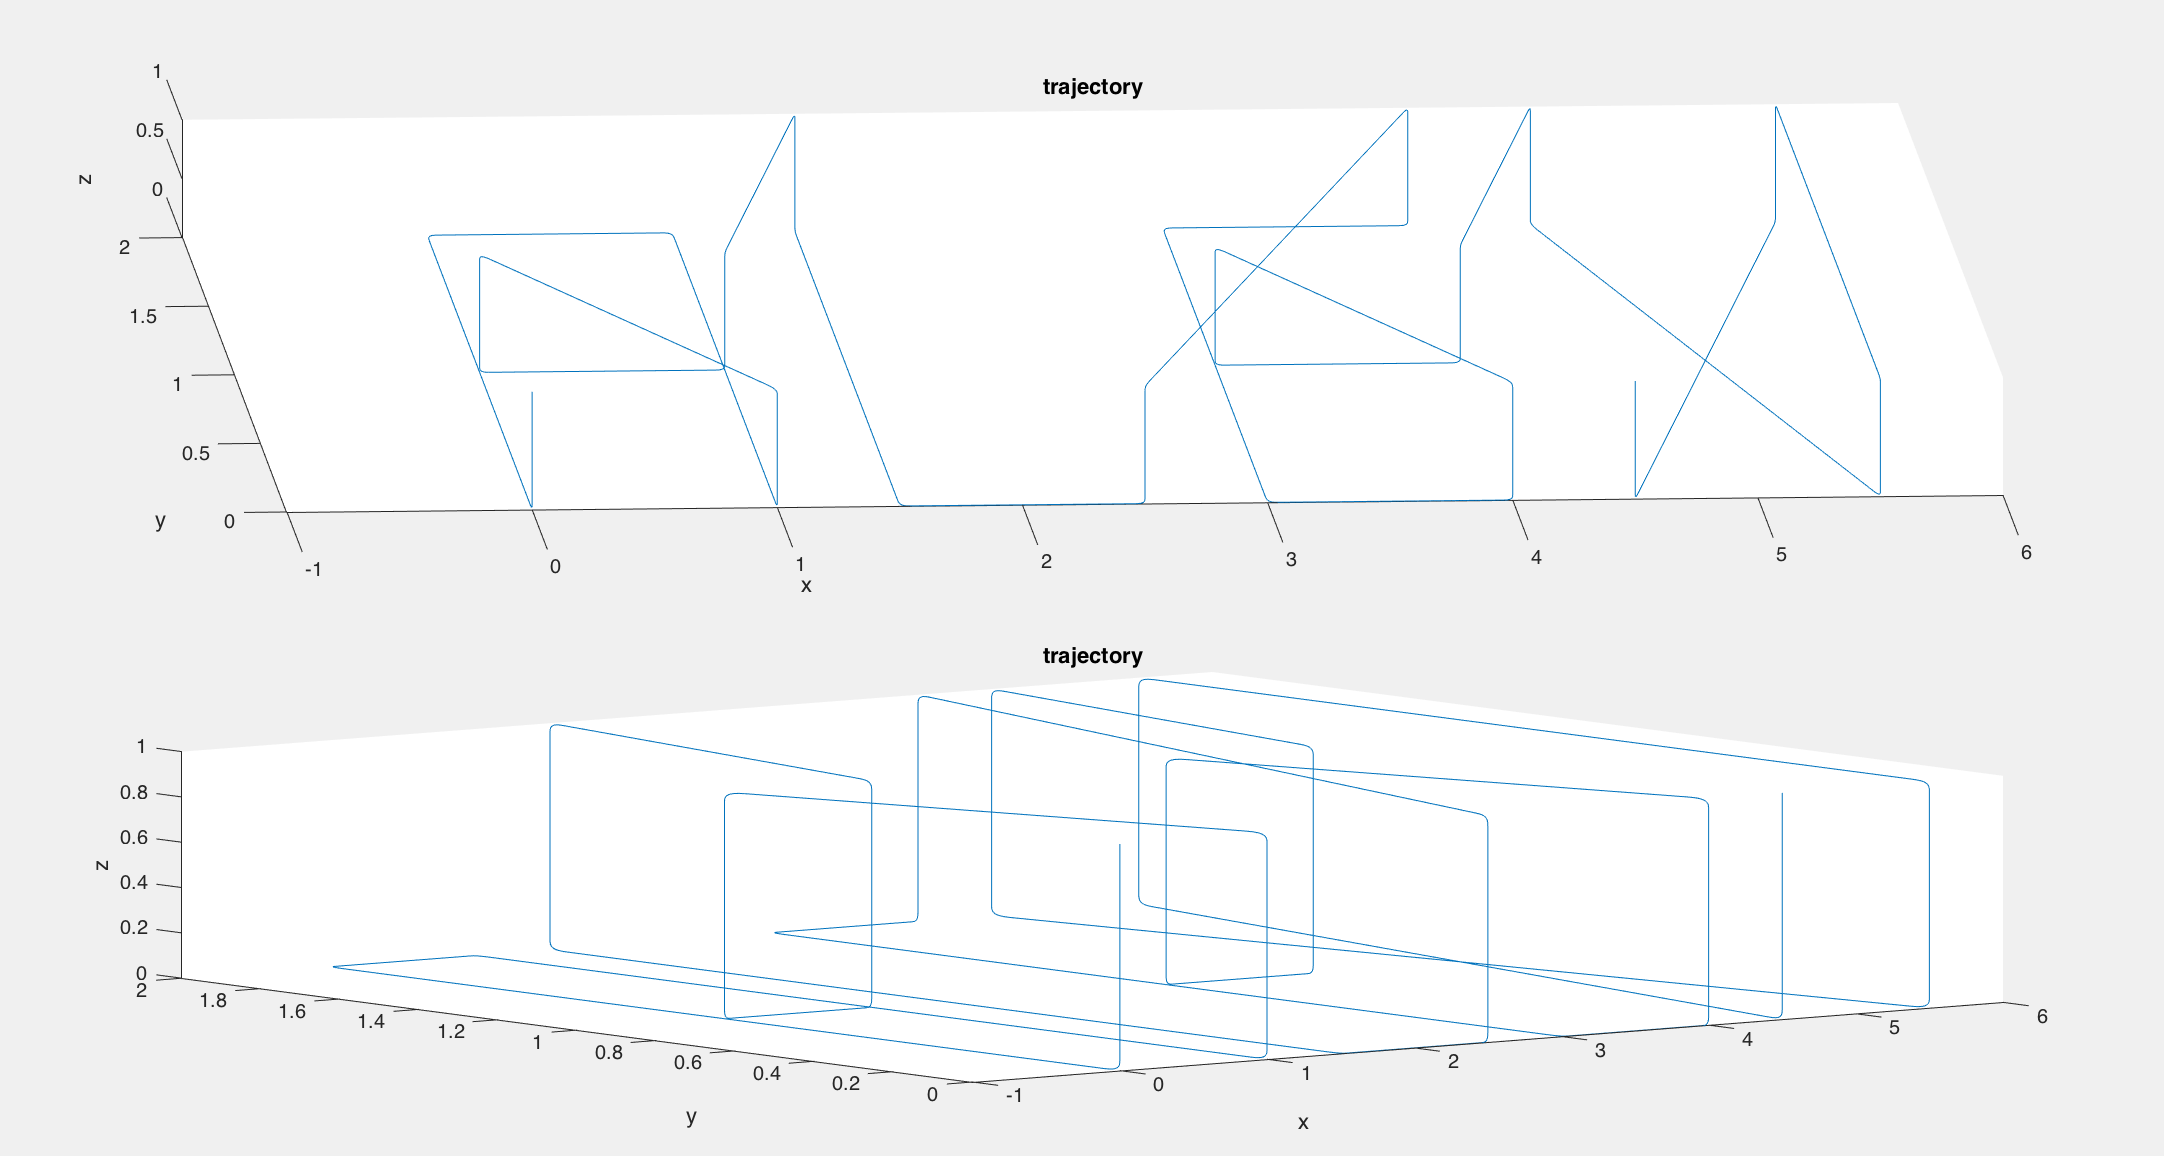
\includegraphics[width=\linewidth]{images/T2}
  \caption{A plot of the end effector trajectory in 3 Dimensions (X,Y,Z)}
  \label{fig:A plot of the end effector trajectory in 3 Dimensions (X,Y,Z)}
\end{figure}

%%%%%%%%%%%%%%%%%%%%%%%%%%%%%%%%%%%%%%%%%%%%%%%%%%%%%%%%%%%%%%%%%%%%%%%%%%%%%%%%%

\section{Part C: Joint Angles with respect to Time}

%\begin{figure}[H]
%  \includegraphics[width=\linewidth]{images/}
%  \caption{A plot showing each of the joint angles with respect to time}
%  \label{fig:A plot showing each of the joint angles with respect to time}
%\end{figure}

%%%%%%%%%%%%%%%%%%%%%%%%%%%%%%%%%%%%%%%%%%%%%%%%%%%%%%%%%%%%%%%%%%%%%%%%%%%%%%%%%

\section{Part D: XYZRPY Magnitudes with respect to Time}

%\begin{figure}[H]
%  \includegraphics[width=\linewidth]{images/}
%  \caption{A plot showing XYZRPY magnitudes with respect to time}
%  \label{fig:A plot showing XYZRPY magnitudes with respect to time}
%\end{figure}

%%%%%%%%%%%%%%%%%%%%%%%%%%%%%%%%%%%%%%%%%%%%%%%%%%%%%%%%%%%%%%%%%%%%%%%%%%%%%%%%%

\section{Part E: choice of trajectory generation technique}

The implementation of the mstraj (Multi-segment multi-axis trajectory) function has been used when creating the path of the trajectory as it has both the properties of the cartesian and joint space method trajectories. Better results are produced when creating curved and straight lines on the x, y and z axis and when approximating fonts there is a more steady range available, for instance the flat head 'A' could be written as a sharpe head or a curved head while maintaining integrity of the path with direct translation instead of pose motion. 

From the information shown on the plots above there are sudden changes in joint angles at = and = which may cause issues with other joints e.g. singularities.

%A brief description (eg. 100 words) of (or justification for) the choice of trajectory generation technique used, its advantages, and limitations.

%%%%%%%%%%%%%%%%%%%%%%%%%%%%%%%%%%%%%%%%%%%%%%%%%%%%%%%%%%%%%%%%%%%%%%%%%%%%%%%%%

\section{Part F}

The mstraj function Produced a good result, and the characters "ALEX" have turned out clear and precise. There is room for improvement as producing scaled and more elegant fonts are optional to an extent based on the constraints of the joint angles. 

When demonstrating this method on a non-virtual machine, it is necessary to take the trajectory limitations from joint angles into account for things such as singularities and overlapping. If there are no other interferences and disturbances in the trajectory the live demo may be accomplished successfully.

%A brief explanation (eg. 100 words) as to whether or not the trajectory is a good one or not (and why). Also briefly mention what would need to be considered before running the trajectory on a real robot.

%%%%%%%%%%%%%%%%%%%%%%%%%%%%%%%%%%%%%%%%%%%%%%%%%%%%%%%%%%%%%%%%%%%%%%%%%%%%%%%%%

\section{Video Demo}

Please find A video demonstration of the Puma 560 trajectory for "ALEX" in the local directory saved as "Demo.mp4"

%%%%%%%%%%%%%%%%%%%%%%%%%%%%%%%%%%%%%%%%%%%%%%%%%%%%%%%%%%%%%%%%%%%%%%%%%%%%%%%%%
%%%%%%%%%%%%%%%%%%%%%%%%%%%%%%%%%%%%%%%%%%%%%%%%%%%%%%%%%%%%%%%%%%%%%%%%%%%%%%%%%


\nocite{*}
\bibliographystyle{ieeetr}
\bibliography{references}
$http://petercorke.com/Robotics_Toolbox.html$
\\
Stevens Lecture Notes Part B (Peter Corke - Chap 7 - Second Half)
\\
Stevens Lecture Notes Part A (Peter Corke - Chap 7 - First Half)
\\
Stevens Lecture Notes Part C (Peter Corke - Chap 8)
\\
Stevens Lecture Notes Part D (Peter Corke - Chap 9 - First Half)

%%%%%%%%%%%%%%%%%%%%%%%%%%%%%%%%%%%%%%%%%%%%%%%%%%%%%%%%%%%%%%%%%%%%%%%%%%%%%%%%
%%%%%%%%%%%%%%%%%%%%%%%%%%%%%%%%%%%%%%%%%%%%%%%%%%%%%%%%%%%%%%%%%%%%%%%%%%%%%%%%

%\clearpage
\section*{APPENDIX}

\begin{lstlisting}[language = C++]



\end{lstlisting}

\end{document}
